% Presentation flag: uncomment to enable presentation features (slower compilation)
\newcommand*{\PRESENTATION}

% Preliminaries
\ifdefined\PRESENTATION
	\documentclass[t]{beamer}
\else
	\documentclass[t,handout]{beamer}
\fi
\mode<presentation>
\usetheme{Warsaw}
\useoutertheme{infolines} 

% Includes
\usepackage{lmodern}
\usepackage{amsmath}
\usepackage{amsfonts}
\usepackage{bbm}
\usepackage{nicefrac}
\usepackage{color}
\usepackage{perpage}
\usepackage{multicol}
\usepackage{tikz}
\usepackage{tikz-dependency}
\usetikzlibrary{graphs,graphs.standard,graphdrawing,quotes,shapes}
\usegdlibrary{layered}

\MakePerPage{footnote}

% Outline slides
\AtBeginSection
{\begin{frame} \frametitle{Outline} \tableofcontents[currentsection,currentsubsection] \end{frame}}
\AtBeginSubsection
{\begin{frame} \frametitle{Outline} \tableofcontents[currentsection,currentsubsection] \end{frame}}


\begin{document}

\title[]{Universal Semantic Parsing with Neural Networks}
\author{Daniel Hershcovich}
\institute[]{PhD Committee Meeting}
\date{October 25, 2016}

\begin{frame}
\titlepage
\end{frame}


\section{Semantic Annotation Schemes}

\begin{frame}
\frametitle{Semantic Annotation Schemes}
\begin{itemize}
 \item Semantic Role Labeling
 \item Semantic Dependencies
 \item Abstract Meaning Representation
 \item Universal Conceptual Cognitive Annotation
\end{itemize}
\end{frame}

\begin{frame}
\frametitle{Semantic Role Labeling (SRL)}
\centering
\vspace*{\fill}
{\color{blue} PropBank}
\vspace*{\fill}

\begin{dependency}
	\begin{deptext}[column sep=1.5em,ampersand replacement=\^]
	After \^ graduation \^ , \^ John \^ moved \^ to \^ Paris \\
	\end{deptext}
	% PropBank
	\node[xshift=4.91em,yshift=3em,color=blue]{move.01}
	child{node at ($(\wordref{1}{5})$) {}};
	\node[xshift=-9.5em,yshift=3em,color=blue]{AM-TMP}
	child{node at ($(\wordref{1}{1})$) {}}
	child{node at ($(\wordref{1}{2})$) {}};
	\node[xshift=.65em,yshift=3em,color=blue]{A1}
	child{node at ($(\wordref{1}{4})$) {}};
	\node[xshift=10.5em,yshift=3em,color=blue]{A2}
	child{node at ($(\wordref{1}{6})$) {}}
	child{node at ($(\wordref{1}{7})$) {}};
	% FrameNet
	\node[xshift=4.91em,yshift=-3em,color=red]{Motion}
	child{node at ($(\wordref{1}{5})$) {}};
	\node[xshift=-9.5em,yshift=-3em,color=red]{Time}
	child{node at ($(\wordref{1}{1})$) {}}
	child{node at ($(\wordref{1}{2})$) {}};
	\node[xshift=.65em,yshift=-3em,color=red]{Theme}
	child{node at ($(\wordref{1}{4})$) {}};
	\node[xshift=10.5em,yshift=-3em,color=red]{Goal}
	child{node at ($(\wordref{1}{6})$) {}}
	child{node at ($(\wordref{1}{7})$) {}};
\end{dependency}

\vspace*{\fill}
{\color{red} FrameNet}
\end{frame}

\begin{frame}
\frametitle{Semantic Dependency Parsing (SDP)}
\centering
\vspace*{\fill}
{\color{blue} DELPH-IN MRS-derived bi-lexical dependencies (DM)}
\vspace*{\fill}

\begin{dependency}[theme=simple]
	\begin{deptext}[column sep=1.5em,ampersand replacement=\^]
	After \^ graduation \^ , \^ John \^ moved \^ to \^ Paris \\
	\end{deptext}
	\deproot{5}{\color{blue} top}
	\depedge{1}{2}{\color{blue} ARG2}
	\depedge{1}{5}{\color{blue} ARG1}
	\depedge{5}{4}{\color{blue} ARG1}
	\depedge{6}{5}{\color{blue} ARG1}
	\depedge{6}{7}{\color{blue} ARG2}
	\deproot[edge below]{5}{\color{red} top}
	\depedge[edge below]{5}{2}{\color{red} TWHEN}
	\depedge[edge below]{5}{4}{\color{red} ACT-arg}
	\depedge[edge below]{5}{7}{\color{red} DIR3-arg}
\end{dependency}

\vspace*{\fill}
{\color{red} Prague Dependency Treebank tectogrammatical layer (PSD)}
\end{frame}

\begin{frame}
\frametitle{Abstract Meaning Representation (AMR)}
\begin{tikzpicture}
\graph[layered layout, sibling distance=5cm, layer distance=2cm, edges={nodes={sloped}}]{
a4 Paris[as={Paris}, black];
a2 John[as={John}, black];
a1[as={person}, black];
a0[as={move-01}, black];
a3[as={city}, black];
a2[as={name}, black];
a5[as={after}, black];
a4[as={name}, black];
a6[as={graduate-01}, black];

a1 ->  ["name"' above, black] a2;
a0 ->  ["ARG0"' above, black] a1;
a0 ->  ["ARG2"' above, black] a3;
a0 ->  ["time"' above, black] a5;
a3 ->  ["name"' above, black] a4;
a2 ->  ["op1"' above, black] a2 John;
a5 ->  ["op1"' above, black] a6;
a4 ->  ["op1"' above, black] a4 Paris;
};
\draw[->, above, black] (a6) to node[sloped] {ARG0} (a1);
\end{tikzpicture}
\end{frame}

\begin{frame}
\frametitle{Universal Conceptual Cognitive Annotation (UCCA)}
\centering
\vspace*{\fill}
\begin{tikzpicture}[level distance=2cm, sibling distance=25mm, ->]
    \node (ROOT) [fill=black, circle] {}
      child {node (After) {After} edge from parent node[left] {\scriptsize $L$\;}}
      child {node (graduation) [fill=black, circle] {}
      {
        child {node {graduation} edge from parent node[left] {\scriptsize $P$}}
      } edge from parent node[left] {\scriptsize $H$} }
      child {node {,} edge from parent node[right] {\scriptsize $U$}}
      child {node (moved) [fill=black, circle] {}
      {
        child {node (John) {John} edge from parent node[left] {\scriptsize $A$}}
        child {node {moved} edge from parent node[left] {\scriptsize $P$}}
        child {node [fill=black, circle] {}
        {
          child {node {to} edge from parent node[left] {\scriptsize $R$}}
          child {node {Paris} edge from parent node[left] {\scriptsize $C$}}
        } edge from parent node[left] {\scriptsize $A$} }
      } edge from parent node[right] {\scriptsize $H$} }
      ;
    \draw[dashed,->] (graduation) to node [auto] {\scriptsize $A$} (John);
    \node (LKG) at (-1.8,0) [fill=black!20, circle] {};
        \draw[bend right] (LKG) to node [auto, left] {\scriptsize $LR$} (After);
        \draw (LKG) to[out=-60, in=120] node [below] {\scriptsize $LA$\quad\;} (graduation);
        \draw (LKG) to[out=30, in=90] node [above] {\scriptsize $LA$} (moved);
\end{tikzpicture}
\vspace*{\fill}
\end{frame}

\begin{frame}
\frametitle{Structural Properties}
\noindent
(1) non-terminal nodes, (2) reentrancy, (3) discontinuity
\centering
\vspace*{\fill}
\begin{minipage}{.48\linewidth}{\centering
  \begin{tikzpicture}[level distance=12mm, sibling distance=16mm, ->,
      every node/.append style={midway}]
    \node (ROOT) [fill=black, circle] {}
      child {node [fill=black, circle] {}
      {
        child {node {John} edge from parent node[left] {\scriptsize $C$}}
        child {node {and} edge from parent node[left] {\scriptsize $N$}}
        child {node {Mary} edge from parent node[left] {\scriptsize $C$}}
      } edge from parent node[left] {\scriptsize $A$} }
      child {node {went} edge from parent node[left] {\scriptsize $P$}}
      child {node {home} edge from parent node[left] {\scriptsize $A$}}
      ;
  \end{tikzpicture}
  }
\end{minipage}
\hfill
\begin{minipage}{.48\linewidth}{\centering
  \begin{tikzpicture}[level distance=12mm, sibling distance=2cm, ->,
      every node/.append style={midway}]
    \node (ROOT) [fill=black, circle] {}
      child {node {John} edge from parent node[left] {\scriptsize $A$}}
      child {node [fill=black, circle] {}
      {
      	child {node {gave} edge from parent node[left] {\scriptsize $C$}}
      	child {node (everything) {everything} edge from parent[white]}
      	child {node {up} edge from parent node[left] {\scriptsize $C$}}
      } edge from parent node[right] {\scriptsize $P$} }
      ;
    \draw[bend right,->] (ROOT) to[out=-20, in=180] node [left] {\scriptsize $A$} (everything);
  \end{tikzpicture}
  }
\end{minipage}

\vspace{-6mm}
  \begin{tikzpicture}[level distance=12mm, sibling distance=2cm, ->,
      every node/.append style={midway}]
    \node (ROOT) [fill=black, circle] {}
      child {node (John) {John} edge from parent node[left] {\scriptsize $A$}}
      child {node {decided} edge from parent node[left] {\scriptsize $P$}}
      child {node (totakeaquickshower) [fill=black, circle] {}
      {
        child {node {to} edge from parent node[left] {\scriptsize $F$}}
        child {node (takeashower) [fill=black, circle] {}
        {
          child {node {take} edge from parent node[left] {\scriptsize $C$}}
          child {node {a} edge from parent node[right] {\scriptsize $F$}}
          child {node (quick) {quick} edge from parent[white]}
          child {node {shower} edge from parent node[right] {\scriptsize $C$}}
        } edge from parent node[right] {\scriptsize $P$} }
      } edge from parent node[left] {\scriptsize $A$} }
      ;
    \draw[bend left,dashed,->] (takeashower) to node [auto] {\scriptsize $A$} (John);
    \draw[bend left,->] (totakeaquickshower) to node [auto] {\scriptsize $D$} (quick);
  \end{tikzpicture}
\end{frame}


\section[]{UCCA Parsing}

\begin{frame}
\frametitle{Goal 1: UCCA Parser}
Fast and accurate parser supporting UCCA's structural properties.

Impact:
\begin{itemize}
\item New general techniques for broad-coverage parsing.
\item Meaning representation for machine translation and its evaluation.\footnote{
Alexandra Birch, Barry Haddow, Ond\v{r}ej Bojar, and Omri Abend. 2016. HUME: Human UCCA-based
evaluation of machine translation. arXiv preprint arXiv:1607.00030}
\item Semantic features for text understanding based on the graph.
\end{itemize}
\begin{center}
 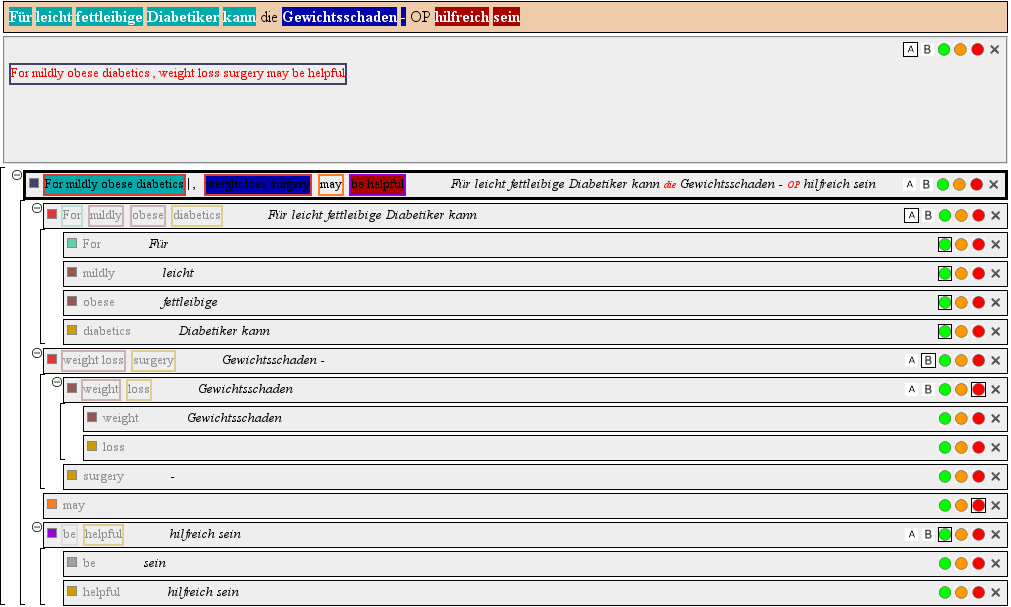
\includegraphics[width=0.6\textwidth,keepaspectratio]{hume}
\end{center}
\end{frame}

\begin{frame}
\frametitle{Transition-Based Parsing}
Parse sentence $w_1 \ldots w_n$ to graph $G=(V,E,\ell)$ incrementally, using buffer $B$ and stack $S$.
\end{frame}


\section[]{Distributed Representation}

\begin{frame}
\frametitle{Goal 2: UCCA-Based Distributed Representation}
Vector representation for sentences and documents,
based on recursive composition on the UCCA graph.

Impact:
\begin{itemize}
\item General automatic semantic feature extractor for text.
\item Accurate measure for text similarity.
\item Understand the semantic contribution of different compositional elements.
\end{itemize}
\end{frame}

\begin{frame}
\frametitle{Recursive Neural Networks}
\end{frame}


\section[]{Applications}

\begin{frame}
\frametitle{Goal 3: Applications}
Use the UCCA parser and distributed representation to improve
performance on semantic tasks:
\begin{itemize}
\item Sentiment analysis.
\item Machine translation.
\item Automatic summarization.
\end{itemize}
\end{frame}


\section[]{Conclusion}

\begin{frame}
\frametitle{Conclusion}
\begin{itemize}
 \item UCCA
\end{itemize}
\end{frame}

\end{document}
